$if(call-to-action)$
% a dashed card centered on the page, like a postcard tucked into the book
\label{call-to-action}
\vspace*{\stretch{1}}
\begin{center}
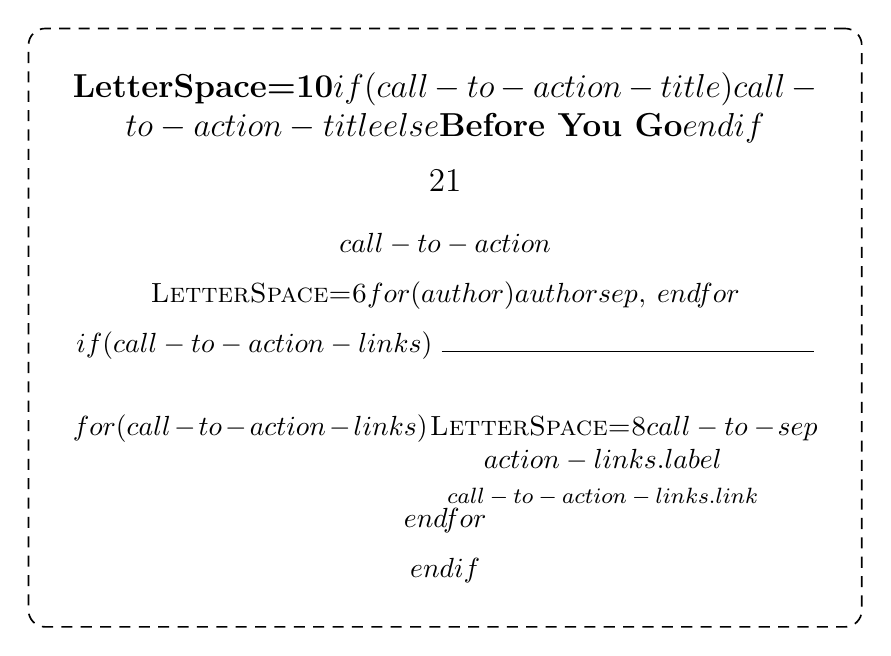
\begin{tikzpicture}
\node[draw, dash pattern=on 4pt off 3pt, line width=0.6pt, rounded corners=6pt, inner sep=16pt]{%
\begin{minipage}{0.78\textwidth}
\centering
\setlength{\parskip}{6pt}
{\chapterheadingfont\bfseries\large\addfontfeature{LetterSpace=10}\MakeTextUppercase{$if(call-to-action-title)$$call-to-action-title$$else$Before You Go$endif$}\par}
{\large\adforn{21}\par}
\vspace{4pt}
$call-to-action$\par
{\scshape\addfontfeature{LetterSpace=6}\MakeTextLowercase{$for(author)$$author$$sep$, $endfor$}\par}
$if(call-to-action-links)$
\vspace{8pt}
{\rule{0.5\linewidth}{0.4pt}\par}
\vspace{4pt}
% links sit side by side, two to a row
$for(call-to-action-links)$\parbox[t]{0.47\linewidth}{\centering{\scshape\addfontfeature{LetterSpace=8}\MakeTextLowercase{$call-to-action-links.label$}\par}\vspace{3pt}{\footnotesize $call-to-action-links.link$\par}}$sep$\hfill$endfor$\par
$endif$
\end{minipage}};
\end{tikzpicture}
\end{center}
\vspace*{\stretch{1}}
$endif$
